\documentclass[conference]{IEEEtran}

\usepackage{cite}
\usepackage{graphicx}
\usepackage{tikz}
\usepackage{pgfplots}
\usepgfplotslibrary{groupplots}
\usetikzlibrary{matrix}
\pgfplotsset{compat=newest}


%\usepackage[cmex10]{amsmath}
% A popular package from the American Mathematical Society that provides
% many useful and powerful commands for dealing with mathematics. If using
% it, be sure to load this package with the cmex10 option to ensure that
% only type 1 fonts will utilized at all point sizes. Without this option,
% it is possible that some math symbols, particularly those within
% footnotes, will be rendered in bitmap form which will result in a
% document that can not be IEEE Xplore compliant!
%
% Also, note that the amsmath package sets \interdisplaylinepenalty to 10000
% thus preventing page breaks from occurring within multiline equations. Use:
%\interdisplaylinepenalty=2500
% after loading amsmath to restore such page breaks as IEEEtran.cls normally
% does. amsmath.sty is already installed on most LaTeX systems. The latest
% version and documentation can be obtained at:
% http://www.ctan.org/tex-archive/macros/latex/required/amslatex/math/


%\usepackage{eqparbox}
% Also of notable interest is Scott Pakin's eqparbox package for creating
% (automatically sized) equal width boxes - aka "natural width parboxes".
% Available at:
% http://www.ctan.org/tex-archive/macros/latex/contrib/eqparbox/


\hyphenation{op-tical net-works semi-conduc-tor}

\begin{document}

\title{Concurrent Patricia Trie \\ \normalsize https://github.com/kl4ng/concurrent-patricia-trie}

\author{\IEEEauthorblockN{Cole Garner}
\IEEEauthorblockA{School of Electrical Engineering and Computer Science\\
University of Central Florida\\
Orlando, Florida 32816\\
Email: ColeGarner@knights.ucf.edu}
\and
\IEEEauthorblockN{Kevin Lang}
\IEEEauthorblockA{School of Electrical Engineering and Computer Science\\
University of Central Florida\\
Orlando, Florida 32816\\
Email: klang2012@gmail.com}}

\maketitle


\begin{abstract}
This paper shows an implementation of a non-blocking Patricia Trie that combines techniques found in numerous recent implementations. It heavily uses the Compare and Swap operation and uses flags to prevent blocking. Additionally, it implements the flags in multiple locations in order to both increase efficiency and reduce the amount of conflicts. It also uses Rust and more efficient memory management and decreased overhead to improve upon its predecessors.
\end{abstract}


\section{Introduction}
A Patricia Trie, also known as a Radix tree, is a unique version of a regular tree. The defining feature of any trie, also known as a digital tree, is that the position of a node in a tree defines the key for that node. A Patricia trie takes this and optimizes the tree by merging any parent node with only one child in order to save space and create a more efficient tree.\cite{Shafiei2013} Because a Patricia Trie is a relatively simple data structure and has many practical uses, it is a good data structure to have an efficient parallelization technique for.
\par
Our implementation of a parallelized, lock-free Patricia Tree will aim to maximize performance and space-efficiency while removing some of the overhead of previous implementations by fine-tuning the memory management. We will combining multiple older approaches and taking the benefits of each and combining them. Our implementation will be focused on using compare-and-swap (CAS) operations which will allow for a blocking-free implementation. \cite{Shafiei2013,Brown2014}
\par
The main changes in our implementation from previous ones is that we will be storing the flags in multiple locations to allow for a smaller portion of the tree to be blocked off for some operations, creating less conflicts overall and increasing performance. \cite{Natarajan2014} The other main improvement we will be making is decreasing the overhead of creating and removing flags by compacting their size as much as possible, and more efficiently handling garbage collection .
\par
Another large difference in our implementation is that we will be using a newer language called Rust and making use of it's unique advantages to help create our more efficient implementation. One benefit Rust offers is that it has an efficient memory-safety property without using garbage collection. However, the largest benefit for our implementation is their unique approach to concurrency using their ownership model that ensures more than one thread can not attempt to write to the same location at the same time. However, just because our specific implementation is in rust does not mean that other languages can not implement the techniques used here.
\par
For the actual Patricia tree algorithm we will be using an algorithm similar to the pseudo-code seen in \cite{Shafiei2013}. However, we will be inserting various improvements on this algorithm, with the main one being that flags will also appear in the edges between two nodes to decrease conflicts. \cite{Natarajan2014}


\section{Related Works}
Creating high-performance, non-blocking data structures has advanced in recent years. There is work into making generalized data structures using CAS operations. \cite{Brown2013} This work has further been expanded into making generalized techniques for non-blocking trees. \cite{Brown2014} These techniques revolve around using load-link extended (LLX), store-conditional extended (SCX) and validate-extended (VLX) primitives which are generalized techniques of the standard, non-extended versions of the primitives. \cite{Brown2013, Brown2014} The techniques used are very powerful and efficient and help form a basis for some techniques used in our work.
\par
Earlier, non-generalized implementation of this technique was seen in a few different data structures. The one related to our work is Shafiei's implementation of non-blocking Patricia Tries. \cite{Shafiei2013} This implementation used a binary tree implementation and handled the parallization by creating flag objects for operations that keep track of what has to be changed. These flags are very powerful because they let multiple threads work on one operation so one thread is not forced to wait. Additionally, since the flag is there there is no chance of a portion of the tree becoming unusable if one thread fails in the middle of an operation. \cite{Shafiei2013, Howley2012} This technique is similar to ours, except we will be eliminating some of the overhead in their implementation due to the large amount of flags they created and the large size of each. Additionally we will be aiming to improve to memory management as compared to it.
\par
A slightly different work is an implementation of a lock-free binary search tree by Natarajan and Mittal. Their work also heavily involves CAS operations but the largest difference is that instead of marking the nodes they mark the edges between the nodes.\cite{Natarajan2014} This has interesting applications in that it allows a smaller portion of the tree to be flagged during insert and delete operations and allows for less conflicts on the whole.
\par
Similar to the previous work is another edge-based algorithm for a concurrent binary search tree by Ramachandran and Mittal. This is not a lock-free solution so it is not completely applicable to ours, however it involves edges and has relatively few nodes locked for each operation. \cite{Ramachandran2015} We will be using some of the techniques used here for the different operations to help further reduce the amount of nodes locked by other implementations and reduce the number of conflicts.
\par
Shun and Blelloch showed another alternative approach to parallization of trees with a multiway Cartesian tree. Theres is slightly unique in that they first create an array and then convert it into a tree. However, despite being different from out project, the algorithms they show in order to generate the tree from the array using parallization techniques warranted study. We looked into their techniques of differentiating what part a particular node is protected in, but ultimately decided the techniques were too far from our own to be much use. \cite{Shun2014}
\par
Due to us implementing this in a way with fully managed memory instead of utilizing a garbage collector, we will be utilizing hazard pointers as initially described by Michael in his seminal 2004 paper. \cite{Michael2004} While the original paper was more oriented towards C++, we will instead be modifying an existing implementation that was found publically available for Rust, extending and modifying it for our own use. \cite{CHAMT}

\section{Rust Language and Libraries}
Rust is a new programming language developed by Mozilla. Developed in parallel with their new Servo web rendering engine, it is developed from the ground up to support safety, concurrency, and parallelism, and was thus a very attractive candidate for our implementation of the concurrent patricia trie.\cite{MozillaResearch} Specifically, in terms of safety it guarantees no data races, buffer or stack overflow, and null pointer exceptions for most use cases. Due to its heavily static nature, it can validate the compiled program to be free of such errors and thus allows us to leverage this in creating a concurrent Patricia trie that has more simple aspects of memory management handled for us. Similarly, it is a language that focuses on speed, which will also help us achieve our desired result of having a Patricia trie implementation that out-performs its counterparts.
\par
However, Rust's approach to memory management, namely it being handled almost entirely by the language without a separate runtime for a garbage collector, has its limits. While this is true for most use cases, it becomes increasingly difficult for the compiler to guarantee this when the complexities of parallel lock-free algorithms come into play. The very nature of these algorithms relies more heavily on complex linearizability reasoning than the compiler can deduce, which means that more complex concurrency problems must have their own memory management, as is in our case.
\par
Since we are building a lock-free data structure with managed memory instead of using a garbage collector, we ended up rolling our own HazardPointer class that will allow us to safely manage memory with no runtime exceptions. The Rust standard library, at the time of this paper, did not have any sort of HazardPointer class for lock-free memory management, which was disappointing since it prides itself on being highly parallelizable and safe. Our implementation is heavily based off one we found implemented for a concurrent hash array mapped trie that was implemented in Rust\cite{CHAMT}, but the code needed to be modified to fit our use case and also because it was no longer properly compiling. This implementation is heavily based on the seminal hazard pointer paper by Michael \cite{Michael2004}, and utilizes recent research in efficient CAS contention management for further improvements.\cite{Dice2013}
\par


\section{Algorithm Description}
Go into detail about what changes (if any) we make from the original pseudocode due to the nature of the Rust language (for better or for worse). Go into detail about what we do new (hopefully able to implement it with more than two children, or have less Flag objects).


\section{Experimental Evaluation}
In this section, we will describe the results of evaluating our edge-based-flagging patricia trie with other similar concurrent data structures.

The other data structures we will be using will be a lock-free binary search tree based on\cite{Natarajan2014} which is also implemented in Java\cite{LFBST}. The second and final data structure we will be testing our results with is a lock-free patricia trie with node-based flagging as described in\cite{Shafiei2013}. For the implementation, we reached out to the author who provided us with his Java source code of his non-replace implementation.

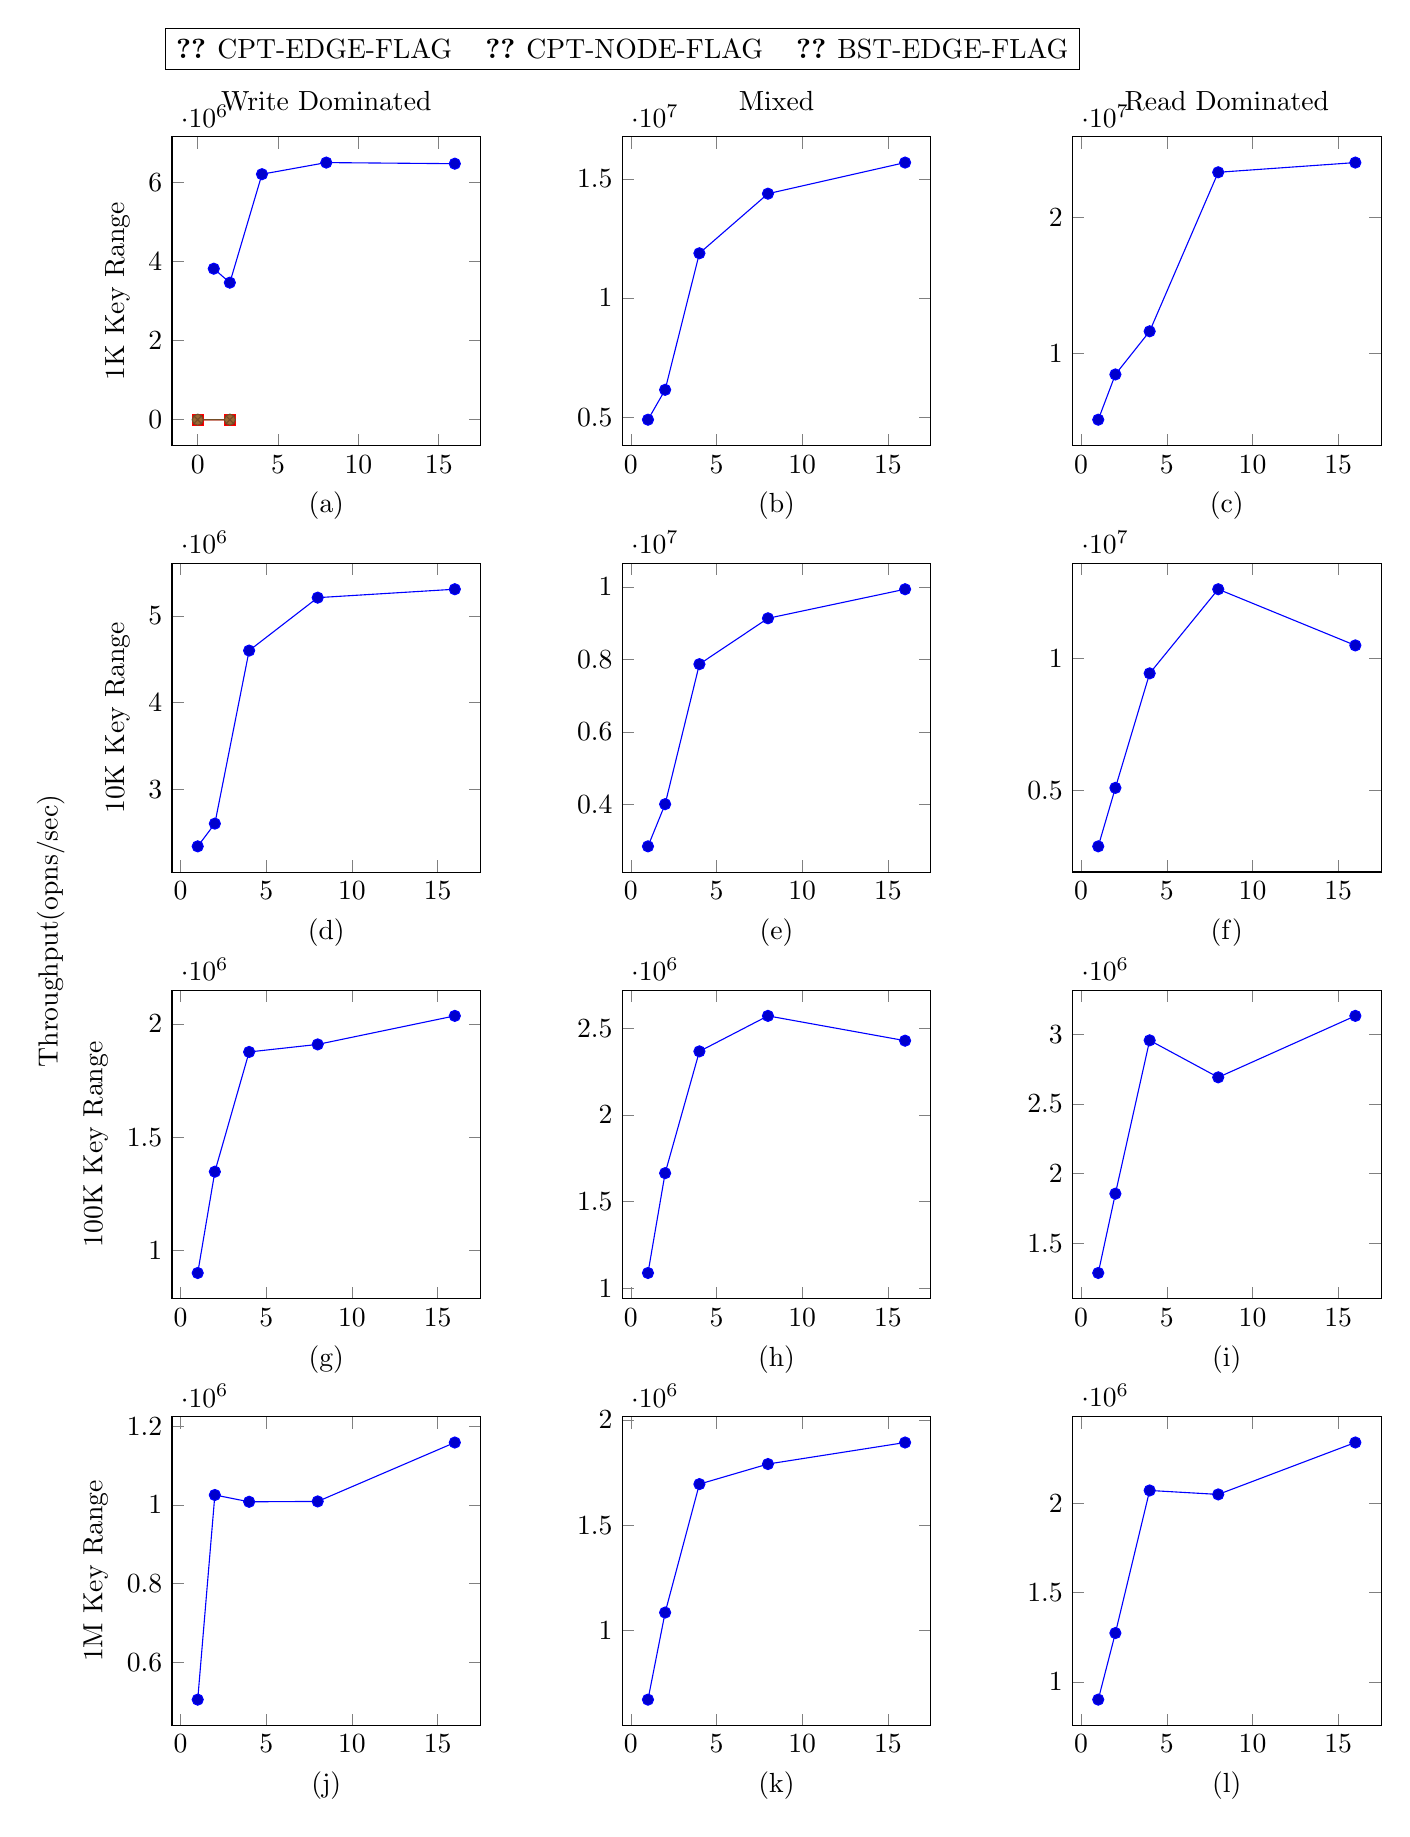
\begin{tikzpicture}
  \begin{groupplot}[group style={group size= 3 by 4, vertical sep=1.5cm, horizontal sep=1.8cm},height=5.5cm,width=5.5cm]
      
      %%
      % 0/50/50 1K
      \nextgroupplot[title=Write Dominated,xlabel={(a)},ylabel={1K Key Range}]
              \addplot coordinates {
                  (1, 3816793.893130) (2, 3463803.255975) (4, 6205398.696866) (8, 6498781.478473) (16, 6470921.297420)
              };\label{plots:cpt-ef}
              \addplot coordinates {
                  (0, 10) (2, 5)
              };\label{plots:cpt-nf}
              \addplot coordinates {
                  (0, 10) (2, 5)
              };\label{plots:bst-ef}
              \coordinate (top) at (rel axis cs:0,1);% coordinate at top of the first plot
      
      % 70/20/10 1K
      \nextgroupplot[title=Mixed,xlabel={(b)}]
              \addplot coordinates {
                  (1, 4892367.906067) (2, 6146281.499693) (4, 11876484.560570) (8, 14378145.219267) (16, 15683199.372672) 
              };\label{plots:cpt-ef}
      
      % 90/9/1 1K
      \nextgroupplot[title=Read Dominated,xlabel={(c)}]
              \addplot coordinates {
                  (1, 5102040.816327) (2, 8431703.204047) (4, 11607661.056297) (8, 23310023.310023) (16, 24024024.024024) 
              };\label{plots:cpt-ef}
      
      %%
      % 0/50/50 10K
      \nextgroupplot[ylabel={10K Key Range},xlabel={(d)}]
              \addplot coordinates {
                  (1, 2341920.374707) (2, 2604166.666667) (4, 4599816.007360) (8, 5210368.633581) (16, 5307503.483049)
              };\label{plots:cpt-ef}
      
      % 70/20/10 10K
      \nextgroupplot[xlabel={(e)}]
              \addplot coordinates {
                  (1, 2842524.161455) (2, 4006410.256410) (4, 7870916.961826) (8, 9136592.051165) (16, 9939122.872407) 
              };\label{plots:cpt-ef}
      
      % 90/9/1 10K
      \nextgroupplot[xlabel={(f)}]
              \addplot coordinates {
                  (1, 2873563.218391) (2, 5089058.524173) (4, 9429514.380009) (8, 12618296.529968) (16, 10489052.051921) 
              };\label{plots:cpt-ef}     
      
      %%
      % 0/50/50 100K
      \nextgroupplot[ylabel={100K Key Range},xlabel={(g)}]
              \addplot coordinates {
                                (1, 900252.070580) (2, 1347708.894879) (4, 1876700.760064) (8, 1910037.245726) (16, 2036037.870304)  
              };\label{plots:cpt-ef}
      
      % 70/20/10 100K
      \nextgroupplot[xlabel={(h)}]
              \addplot coordinates {
                  (1, 1087902.523934) (2, 1664447.403462) (4, 2367704.510477) (8, 2572678.157962) (16, 2429469.464606) 
              };\label{plots:cpt-ef}
      
      % 90/9/1 100K
      \nextgroupplot[xlabel={(i)}]
              \addplot coordinates {
                  (1, 1287001.287001) (2, 1855976.243504) (4, 2956393.200296) (8, 2690884.628322) (16, 3132096.155352) 
              };\label{plots:cpt-ef}
      
      %%
      % 0/50/50 1M
      \nextgroupplot[ylabel={1M Key Range},xlabel={(j)}]
              \addplot coordinates {
                                (1, 504948.495253) (2, 1025325.540859) (4, 1008013.708986) (8, 1008954.470929) (16, 1158731.768080) 
              };\label{plots:cpt-ef}

      % 70/20/10 1M
      \nextgroupplot[xlabel={(k)}]
              \addplot coordinates {
                  (1, 671140.939597) (2, 1084951.719648) (4, 1695489.996609) (8, 1790911.126035) (16, 1893132.661271) 
              };\label{plots:cpt-ef}
      
      % 90/9/1 1M
      \nextgroupplot[xlabel={(l)}]
              \addplot coordinates {
                  (1, 900414.190528) (2, 1273398.701133) (4, 2072753.653228) (8, 2050545.957861) (16, 2341577.637934) 
              };\label{plots:cpt-ef}
              \coordinate (bot) at (rel axis cs:0,0);% coordinate at bottom of the last plot
  \end{groupplot}
  \path (top-|current bounding box.west)-- 
        node[anchor=south,rotate=90] {Throughput(opns/sec)} 
        (bot-|current bounding box.west);
          
  % legend
  \path (top|-current bounding box.north)--
        coordinate(legendpos)
        (bot|-current bounding box.north);
  \matrix[
      matrix of nodes,
      anchor=south,
      draw,
      inner sep=0.2em,
      draw
    ]at([yshift=1ex]legendpos)
    {
      \ref{plots:cpt-ef}& CPT-EDGE-FLAG&[8pt]
      \ref{plots:cpt-nf}& CPT-NODE-FLAG&[8pt]
      \ref{plots:bst-ef}& BST-EDGE-FLAG\\};
\end{tikzpicture}
\clearpage


\section{Conclusion}
The conclusion goes here, once we finish the above sections.


\section{Acknowledgment}
Acknowledge original paper author here once he (hopefully) provides source code and any other Patricia trie implementations we test against for empirical evaluation.


% appendix section for midterm report
\appendix
\subsection{Challenges}
The first challenges we faced was trying to find a suitable C++ stdlib data structure that we could improve in a novel way, but we couldn't find anything where we felt we could make a big enough improvement to be worthwhile to do a semester-long project on. Later on, when we were moving towards doing a more esoteric data structure in any sort of managed-memory language, we found out that one of our group mates decided to drop the class which lead to some further delays as we had to reassess what sort of topics were within our scope when we had less manpower.
\par
As mentioned in the Rust Language section, a large part of the challenges thus far was trying to understand this somewhat esoteric language. Both of us come from a heavy background of Java, where the strict OOP styling in addition to garbage collection made reasoning about memory allocation and management on the stack or heap easy to reason about. However, Rust has a unique memory model where there is not only the distinction between stack and heap, but also between what can and cannot be shared, and what can and cannot be modified. This, combined with our initial lack of familiarity with the memory-related needs of lock-free data structures, like the need for some sort of hazard pointer type for memory management, lead to much of our time just trying to figure out the best way to approach this problem from both the perspective of the language's best practices and the recommendations by the current state of parallel-related academia.
\par
Indeed, until recently it was thought that the Arc data type in the Rust standard library, perhaps combined with the AtomicPtr data type, would be sufficient for our needs, and was a motivator for choosing Rust as the language of implementation as well. However, as we became more familiar with this somewhat sparsely-documented language, it became apparent that a lot of the functionality that drew us towards the language actually became less functional as one moves into more complex parallel algorithms and data structures. Nevertheless, the language has atomic primitives built into it and a thriving community which made finding info on Rust best practices as easy as going to the relevant IRC channel.
\par


\subsection{Completed Tasks}
We have completed practically all research we need in order to not only implement our current vision for this project, which currently is to not only fully implement the structure described by the pseudo-code in the paper we got most of our inspiration from this project from\cite{Shafiei2013}, but also to extend it to >2 children and possibly make further improvements in respects to the flags that facilitate most of the operations on the data structure.
\par
We have also reached out to the author of the aforementioned paper in hopes of obtaining source code to test against in order to see performance gains from using a non-GC and high-performance language, though we have yet to get a response. However, we have found other suitable source codes for this sort of comparison, also written in Java, though seemingly not as up-to-date in terms of utilizing the recent lock-free developments of Patricia tries or any tree in academia.\cite{PATSource}
\par
We have coded up part of the actual algorithm, but recently got blocked by realizing that we needed to roll our own HazardPointer class in order to be able to safely manage memory in this lock-free data structure. However, since we now seem to have a clear and complete vision of the nature of our chosen topic, we plan on being able to complete coding up the binary-version of the concurrent Patricia trie within the coming weeks.
\par


\subsection{Remaining Tasks}
\begin{itemize}
\item Complete basic code for concurrent Patricia tree, based off of \cite{Shafiei2013} pseudocode.
\item Solve any potential issues with rust. Main issue currently is figuring out how to work with Hazard Pointers.
\item Attempt to modify flag structure and how the memory management of it is handled in order to decrease overhead. Instead of letting a garbage collector handle everything, attempt manually managing the memory using Rust and see how the performance compares.
\item Attempt to create additional flag locations in the edges between nodes in order to decrease conflicts and increase efficiency. Test whether flags in only the nodes, only in the edges, or in both depending on the operation is most efficient.
\item Hopefully get the source codes we requested from other papers and further look into their implementations and compare it to ours, and see if there is anything we can do to further improve our implementation.
\item Look into the best ways to compare the performance of our data structures versus other implementations and then actually run the comparisons and document the results.
\item Finish the paper once we have finished everything else.
\end{itemize}


% references section
\bibliographystyle{IEEEtran}
\bibliography{IEEEabrv,references}


\end{document}


%\subsection{Subsection Heading Here}
%Subsection text here.


%\subsubsection{Subsubsection Heading Here}
%Subsubsection text here.
